\documentclass[a4paper]{exam}

\usepackage{graphicx}

\usepackage{siunitx}
\DeclareSIUnit{\revolution}{rev}
\DeclareSIUnit{\rpm}{\revolution\per\minute}
\DeclareSIUnit{\lightyear}{ly}

\begin{document}
  \section*{L2 Physics: Problems on electrodynamics}
  \subsection*{Sections 1.1-1.3}
  Main concepts you should understand: electric field, electrostatic force, electric potential energy, electric potential (voltage).
  \begin{questions}
    \question (NZQA 2018) A Van der Graaf generator is connected to two large metal plates, \SI{0.080}{\metre} apart.
  \end{questions}
  \clearpage
  \section*{Formulae}
  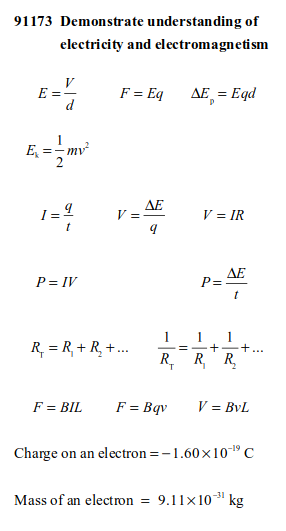
\includegraphics{edyn}
\end{document}
